\documentclass[fleqn]{article}

\usepackage{graphicx}
\usepackage{hyperref}
\usepackage[margin=1.0in]{geometry}
\usepackage{float}
\usepackage{amsmath}

\newcommand{\unit}[1]{\ensuremath{\, \mathrm{#1}}}

\title{\Huge Weighing a Whale}
\author{Nicholas Schweitzer}
\date{}
\setlength\parindent{0pt}
\setlength{\mathindent}{24pt}

\begin{document}
\maketitle

\section{Finding the weight and density of a whale}

\begin{figure}[H]
  Assume the length of the whale in the picture is 14 m long and the length has been measured accurately using drones.

  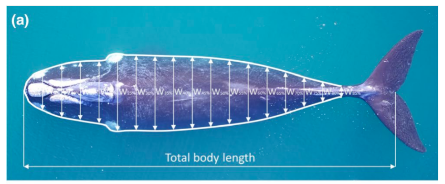
\includegraphics{whale_with_distances.png}
\end{figure}

\href{https://www.bbc.com/news/science-environment-49893849}{https://www.bbc.com/news/science-environment-49893849}
\\\\

\begin{figure}[H]
  \textbf{1.} Add this image to geogebra or desmos and adjust the scale appropriately. Have the horizontal axis of symmetry lie along the x-axis.

  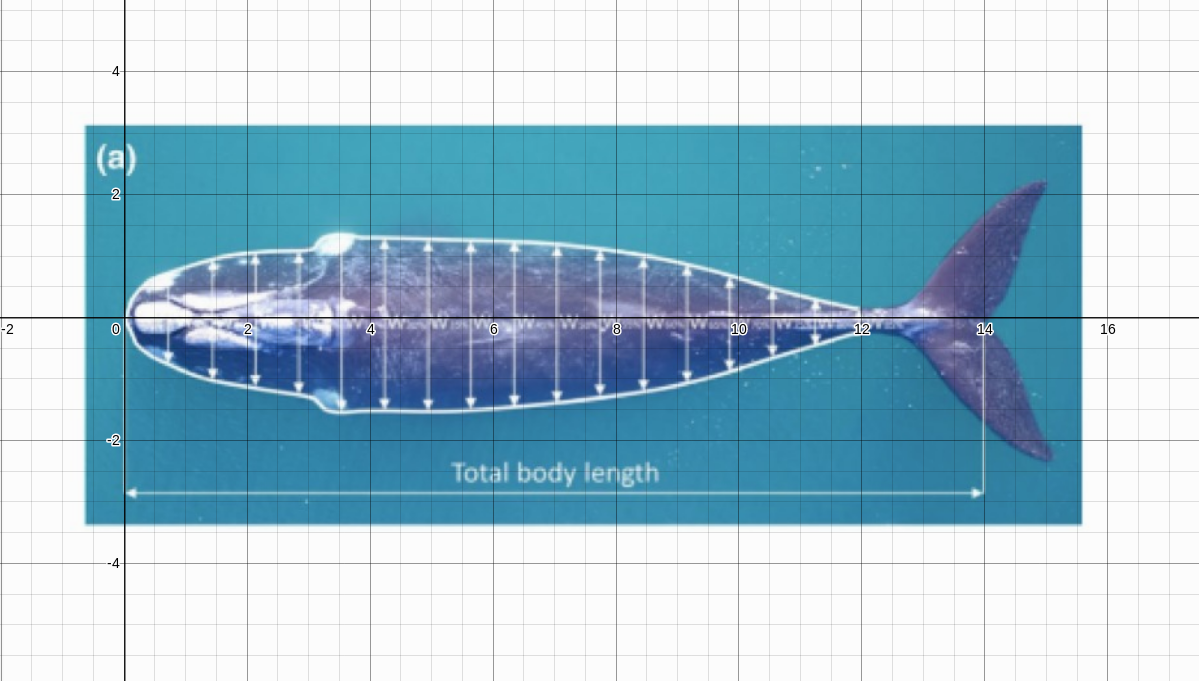
\includegraphics[scale=0.4]{desmos-whale.png}
  The \textbf{girth} of the whale at a given point is the circumference of the circular cross-section at this point.
\end{figure}

\textbf{2.} From your diagram work out an estimate for the maximum girth of the whale.
\begin{equation*}
  d = 2.9\unit{m}
\end{equation*}
\begin{equation*}
  C = \pi d
\end{equation*}
\begin{equation*}
  C = \pi \times 2.9
\end{equation*}
\begin{equation*}
  C \approx 9.11\unit{m}
\end{equation*}
\smallskip

A formula that can approximate the weight (\textit{M}) of a whale from its size is:
\begin{equation*}
  M = 6,144.79 - 1,788B - 914C_{40\%}+500BC_{40\%}
\end{equation*}
\smallskip

\textbf{3.} Use the formula to estimate the weight of the whale.
\begin{equation*}
  B = 14\unit{m}
\end{equation*}
\begin{equation*}
  C_{40\%} = 9.11\unit{m}
\end{equation*}
\begin{equation*}
  M = 6,144.79 - 1,788B - 914C_{40\%}+500BC_{40\%}
\end{equation*}
\begin{equation*}
  M = 6,144.79 - 1,788 \times 14 - 914 \times 9.11 + 500 \times 14 \times 9.11
\end{equation*}
\begin{equation*}
  M \approx 36.556
\end{equation*}
\smallskip

In order to find the average density of a whale an estimate for the volume needs to be calculated.

\textbf{4.}	Find an equation (or equations) that models the upper half of the body of the whale.

\textbf{5.}	Use a spreadsheet and your model to estimate the distance from the line of symmetry of the whale to the upper edge at intervals of 25 cm.

\textbf{6.}	Find an estimate for the volume of the whale and hence its density.  

For question 6 you should assume the cross-section of the whale is circular (up to the start of the tail).

	Does your answer make sense in the context of the problem?

\textbf{7.}	Discuss 

a	The issues particular to the real life problem which may have led to inaccuracies in your answer.  Try to quantify these eg are they likely to lead to your answer being an underestimate or an overestimate?

b	Consider the mathematical process used to find the density of the whale.  Which part of the process might lead to inaccuracies in your answer?  Can you quantify these at all?  How might you improve the process to achieve a more accurate answer?

\textbf{8.}	Address one of the sources of error mentioned in question 7 and  try to account for it to achieve an improved estimate.


\section{Section 2}

Use mathematics to find an estimate for the surface area of a whale or a sea creature of your choosing. 

Your process should include an initial answer and then an identification of an improvement that could be made, which is then carried out.

Clearly explain all your steps  and discuss, as precisely as you can, any limitations of the process.  
\end{document}
